\documentclass[margin=2mm]{standalone}
\usepackage{tikz-sections}

\begin{document}
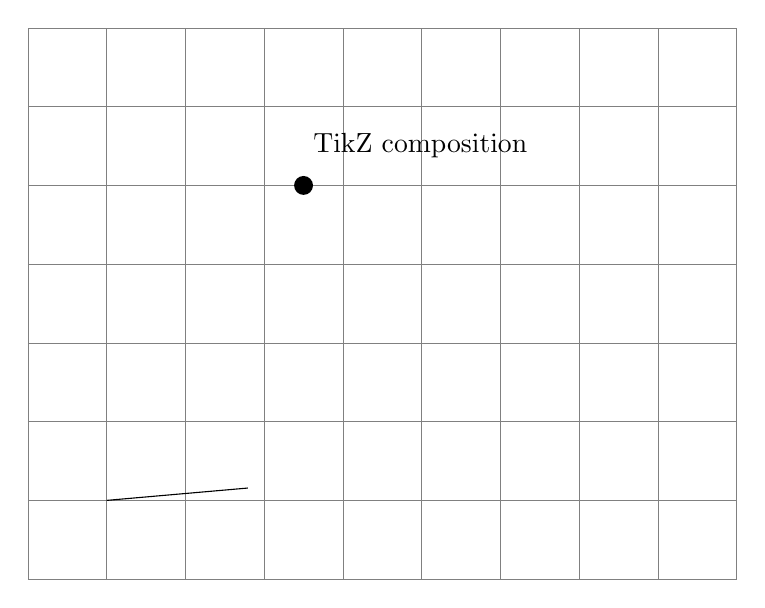
\begin{tikzpicture}[x=1mm,y=1mm]
  \draw[help lines, step=10] (-10,-10) grid (80,60);

  \begin{scope}[shift={(0,0)}, rotate=5]
    \TikZSectionsLippedChannel[
      depth=120,
      flange=40,
      lip=12,
      thickness=2,
      inside radius=3,
      scale=0.12
    ]
    \draw[black] (0,0) -- (18,0);
  \end{scope}

  \begin{scope}[shift={(35,0)}, xscale=-1]
    \TikZSectionsZee[
      depth=100,
      flange=35,
      thickness=2,
      bend radius=3,
      scale=0.12
    ]
  \end{scope}

  \TikZSectionsRHS[
    depth=80,
    width=50,
    thickness=3,
    root radius=4,
    at={(42,4)},
    scale=0.12,
    rotate=12,
    xscale=1.2,
    yscale=0.8,
    filled=true
  ]

  \TikZSectionsCHS[
    radius=18,
    thickness=2,
    at={(4,34)},
    scale=0.18,
    centerline=true,
    dimensions=true
  ]

  \node[anchor=west] at (25,45) {TikZ composition};
  \fill[black] (25,40) circle[radius=1.2];
\end{tikzpicture}
\end{document}
